\chapter*{La Música y las Frecuencias}
\addcontentsline{toc}{chapter}{La Música y las Frecuencias}
\markboth{La Música y las Frecuencias}{La Música y las Frecuencias}
\vspace{0.6cm}
\begin{center}
\nopagebreak
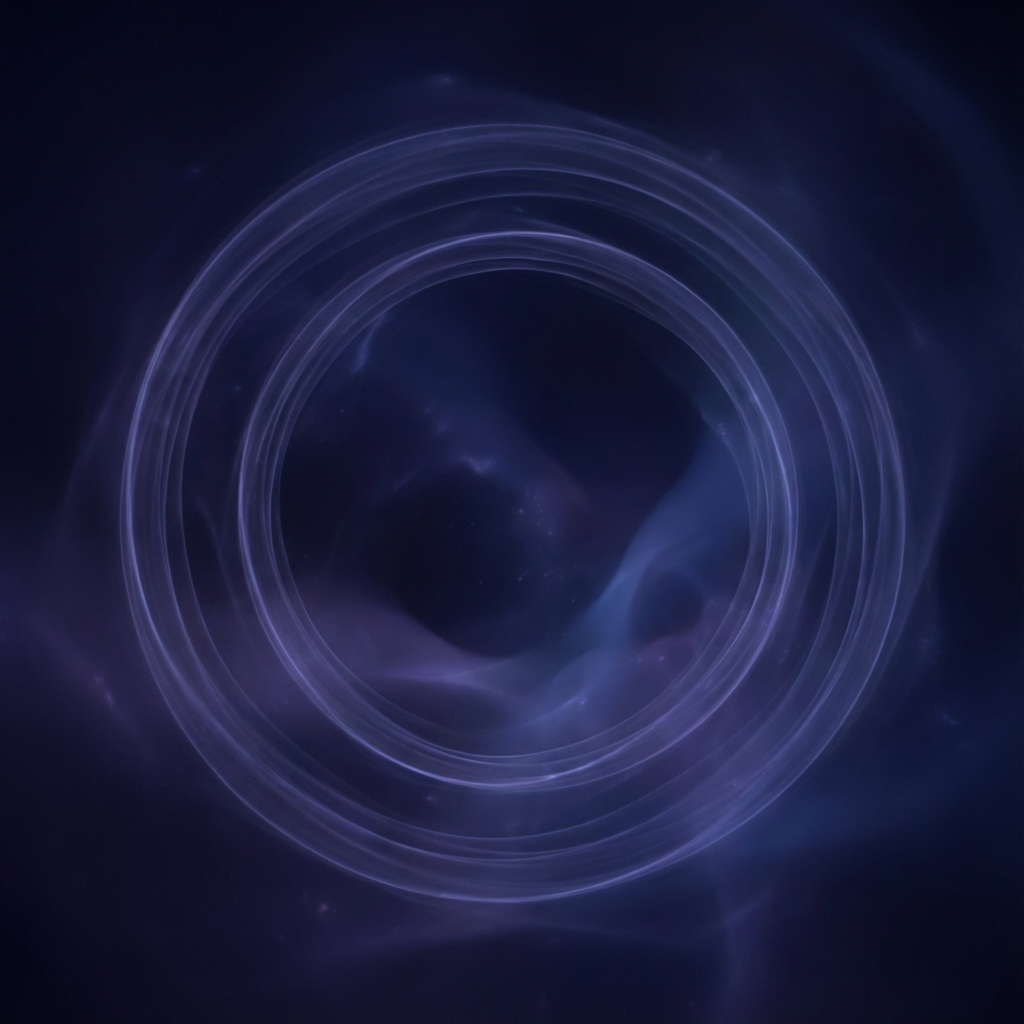
\includegraphics[width=0.75\textwidth,cfbox=gray!60 0.6pt 4pt]{silence_vibration.png}\\
\vspace{4pt}
{\small\itshape La música y el arte: vehículos directos de alta vibración.}
\end{center}

\vspace{0.6cm}
La experiencia de \textit{Mi Amigo Jesucristo} no termina en las palabras escritas: fue concebida desde su origen como una \textbf{obra multisensorial y vibratoria}, donde el sonido actúa como vehículo directo de sintonización interior.


\vspace{0.4cm}
\begin{center}
\rule{0.35\textwidth}{0.4pt}
\end{center}
\vspace{0.4cm}


\subsection*{La Creación Musical de Maria Paz Arés Osset}
Cada capítulo del libro resuena con composiciones musicales y frecuencias sonoras creadas por \textbf{Maria Paz Arés Osset}. Estas melodías están diseñadas para acompañar la mente y el corazón en un estado de relajación profunda, coherencia y apertura.

Al escuchar estas piezas musicales:
\noindent\textbullet~~\textbf{El ritmo cerebral disminuye} hacia estados alfa y theta, facilitando la introspección y la paz.\\

\noindent\textbullet~~\textbf{Se disuelven las tensiones} y las cargas emocionales densas acumuladas en el día a día.\\

\noindent\textbullet~~\textbf{El mensaje del texto se integra} a nivel subconsciente y celular a través del lenguaje universal del sonido.\\



\vspace{0.4cm}
\begin{center}
\rule{0.35\textwidth}{0.4pt}
\end{center}
\vspace{0.4cm}


\subsection*{Cómo Vivir la Experiencia Sonora}
Te invitamos a escuchar el álbum mientras lees cada capítulo o durante tus momentos diarios de meditación y silencio:
\noindent\textbf{1.}~~\textbf{En Spotify}: Puedes buscar las pistas oficiales del álbum y sumergirte en sus atmósferas envolventes.\\

\noindent\textbf{2.}~~\textbf{En la Web Oficial}: Visita [pazaresosset.es](https://pazaresosset.es) para acceder a todas las novedades, arte visual y material adicional de la autora.\\




\begin{quote}
\itshape \textit{«La música es la voz del alma que recuerda a la materia su origen de pura Luz.»}
\end{quote}

\vspace{1.5cm}
\begin{center}
\textit{Para completar esta experiencia vibracional, te invito a seguir los enlaces y sumergirte en la música del libro.}\\
\vspace{1cm}
\begin{minipage}{0.45\textwidth}
\centering
\qrcode[height=3.2cm]{https://open.spotify.com/album/6FkbQuY2d7F09zmG2hqnFK}\\
\vspace{0.4cm}\textbf{Escuchar en Spotify}
\end{minipage}\hfill
\begin{minipage}{0.45\textwidth}
\centering
\qrcode[height=3.2cm]{https://pazaresosset.es}\\
\vspace{0.4cm}\textbf{pazaresosset.es}
\end{minipage}
\end{center}